\documentclass[a4paper,twoside,master.tex]{subfiles}
\begin{document}
\lecture{28}{Wednesday, October 23, 2019}{Square Well Potential}

Let's examine the steady state wave function solutions for a square well:
\begin{equation}
    V =
    \begin{cases} 
        V_0 & x < -a/2\\
        0 & -a/2<x<a/2\\
        V_0 & a/2 < x
    \end{cases}
\end{equation}
For a steady state, recall that we generally want
\begin{equation}
    \varphi(x,t) = e^{- \imath E t / \hbar} \varphi(x)
\end{equation}
Now we can use the time independent Schr\"odinger equation:
\begin{equation}
    H \varphi = E \varphi
\end{equation}
where
\begin{equation}
    H = \frac{P^2}{2m} + V(x)
\end{equation}
so
\begin{equation}
    - \partial_x^2 \varphi(x)  = \left( \frac{2m}{\hbar} \right)(E-V(x)) \varphi(x)
\end{equation}

In the regions with a nonzero potential, recall that we say the solution looks like $ e^{\pm \kappa x} $. On the left side, we want this to be $ + $ and on the right we want $ - $ so that we don't get wave functions which diverge at infinity. In the middle, the wave function looks like $ e^{\pm \imath k x} $.

Our potential is symmetric under parity: $ V(x) = V(-x) $, so the parity operator $ \Pi $ commutes with the Hamiltonian: $ \comm{H}{\Pi} =0 $. The parity operator forms a group with two elements, $ G = \{e, \Pi\} $, where $ e $ is the identity. Applying the group operator twice returns us to the original state. One of the consequences of this symmetry is that, when we solve the Schr\"odinger equation and find some solution,
\begin{equation}
    H \ket{\varphi} E \ket{\varphi}
\end{equation}
because $ \Pi H \Pi^\dagger = H $, we know that
\begin{align}
    \Pi H \Pi^{-1} \Pi \ket{\varphi} &= \Pi E \ket{\varphi}\\
    H(\Pi \ket{\varphi})= E(\Pi \ket{\varphi})
\end{align}
This means that if we find an eigenstate of the Hamiltonian, we can apply the parity operator to our solution and get another solution with the same energy. Sometimes these will be the same solution.

\begin{note}{Important Idea}
    We can do this same trick with \textit{any} operator which commutes with the Hamiltonian. Eigenfunctions of the Hamiltonian are ``basis'' functions of representation of $ G $, the symmetry group of the Hamiltonian.
\end{note}

For this group $ G $, $ \Pi = 
\begin{bmatrix}
    () & 0\\
    0 & ()
\end{bmatrix}
$, and $ \Pi^2 = e $ so the eigenvalues must be $ \pm 1 $. This means there is a basis where the parity operator is
\begin{equation}
    \Pi = 
    \begin{bmatrix}
        1 & 0\\
        0 & -1
    \end{bmatrix}
\end{equation}
so there exist eigenstates $ \ket{\varphi_\pm} $ such that
\begin{equation}
    \Pi \ket{\varphi_+} = \ket{\varphi_+}
\end{equation}
and
\begin{equation}
    \Pi \ket{\varphi_-} = - \ket{\varphi_-}
\end{equation}
Unfortunately, applying the operator in our case will not give us a new solution, but it does tell us that we must have one even solution and one odd solution. Let's look at $ \varphi_+(x) $:
\begin{equation}
    \varphi_+(x) =
    \begin{cases}
        A e^{-\kappa x} & a/2 < x\\
        B \cos(kx) & -a/2 < x < a/2\\
        Ae^{+ \kappa x} & x < -a/2
    \end{cases}
\end{equation}
Note the symmetry in coefficients. Now let's look at the other solution:
\begin{equation}
    \varphi_-(x) =
    \begin{cases} 
        A e^{-\kappa x} & a/2 < x\\
        B \sin(kx) & -a/2 < x < a/2\\
        -A e^{+\kappa x} & x < -a/2
    \end{cases}
\end{equation}

Putting these solutions back into the Schr\"odinger equation, we find that $ k = \sqrt{2mE/ \hbar^2} $ and $ \kappa = \sqrt{2m (V_0 - E)/ \hbar^2} $. Now we know almost everything about our solutions except for $ A $ and $ B $. The important condition is at the boundaries, where we must preserve continuity of the wave function and its derivative. For $ \varphi_+ $, we find that, at the right-hand boundary,
\begin{equation}
    B \cos(k a/2) = A e^{- \kappa a/2}
\end{equation}
For the derivative,
\begin{equation}
    -kB \sin(k a/2) = - \kappa A e^{- \kappa a/2}
\end{equation}
Let's divide the bottom equation by the top equation. This gives us
\begin{equation}
    \tan(k a/2) = \frac{\kappa}{k}
\end{equation}
We were trying to find a relation between $ A $ and $ B $, but we have now found a relationship between $ k $ and $ \kappa $! Notice as we vary the energy $ E $, both $ k $ and $\kappa$ vary continuously. The tangent equation does not hold for every $ k $ and $\kappa$, but we can imagine that there will be some values which work. Let's try to figure out what this means. Notice on the left-hand side, the function is transcendental, so this will be a difficult equation to solve. We look for a graphical solution:

\begin{figure}[h]
    \centering
    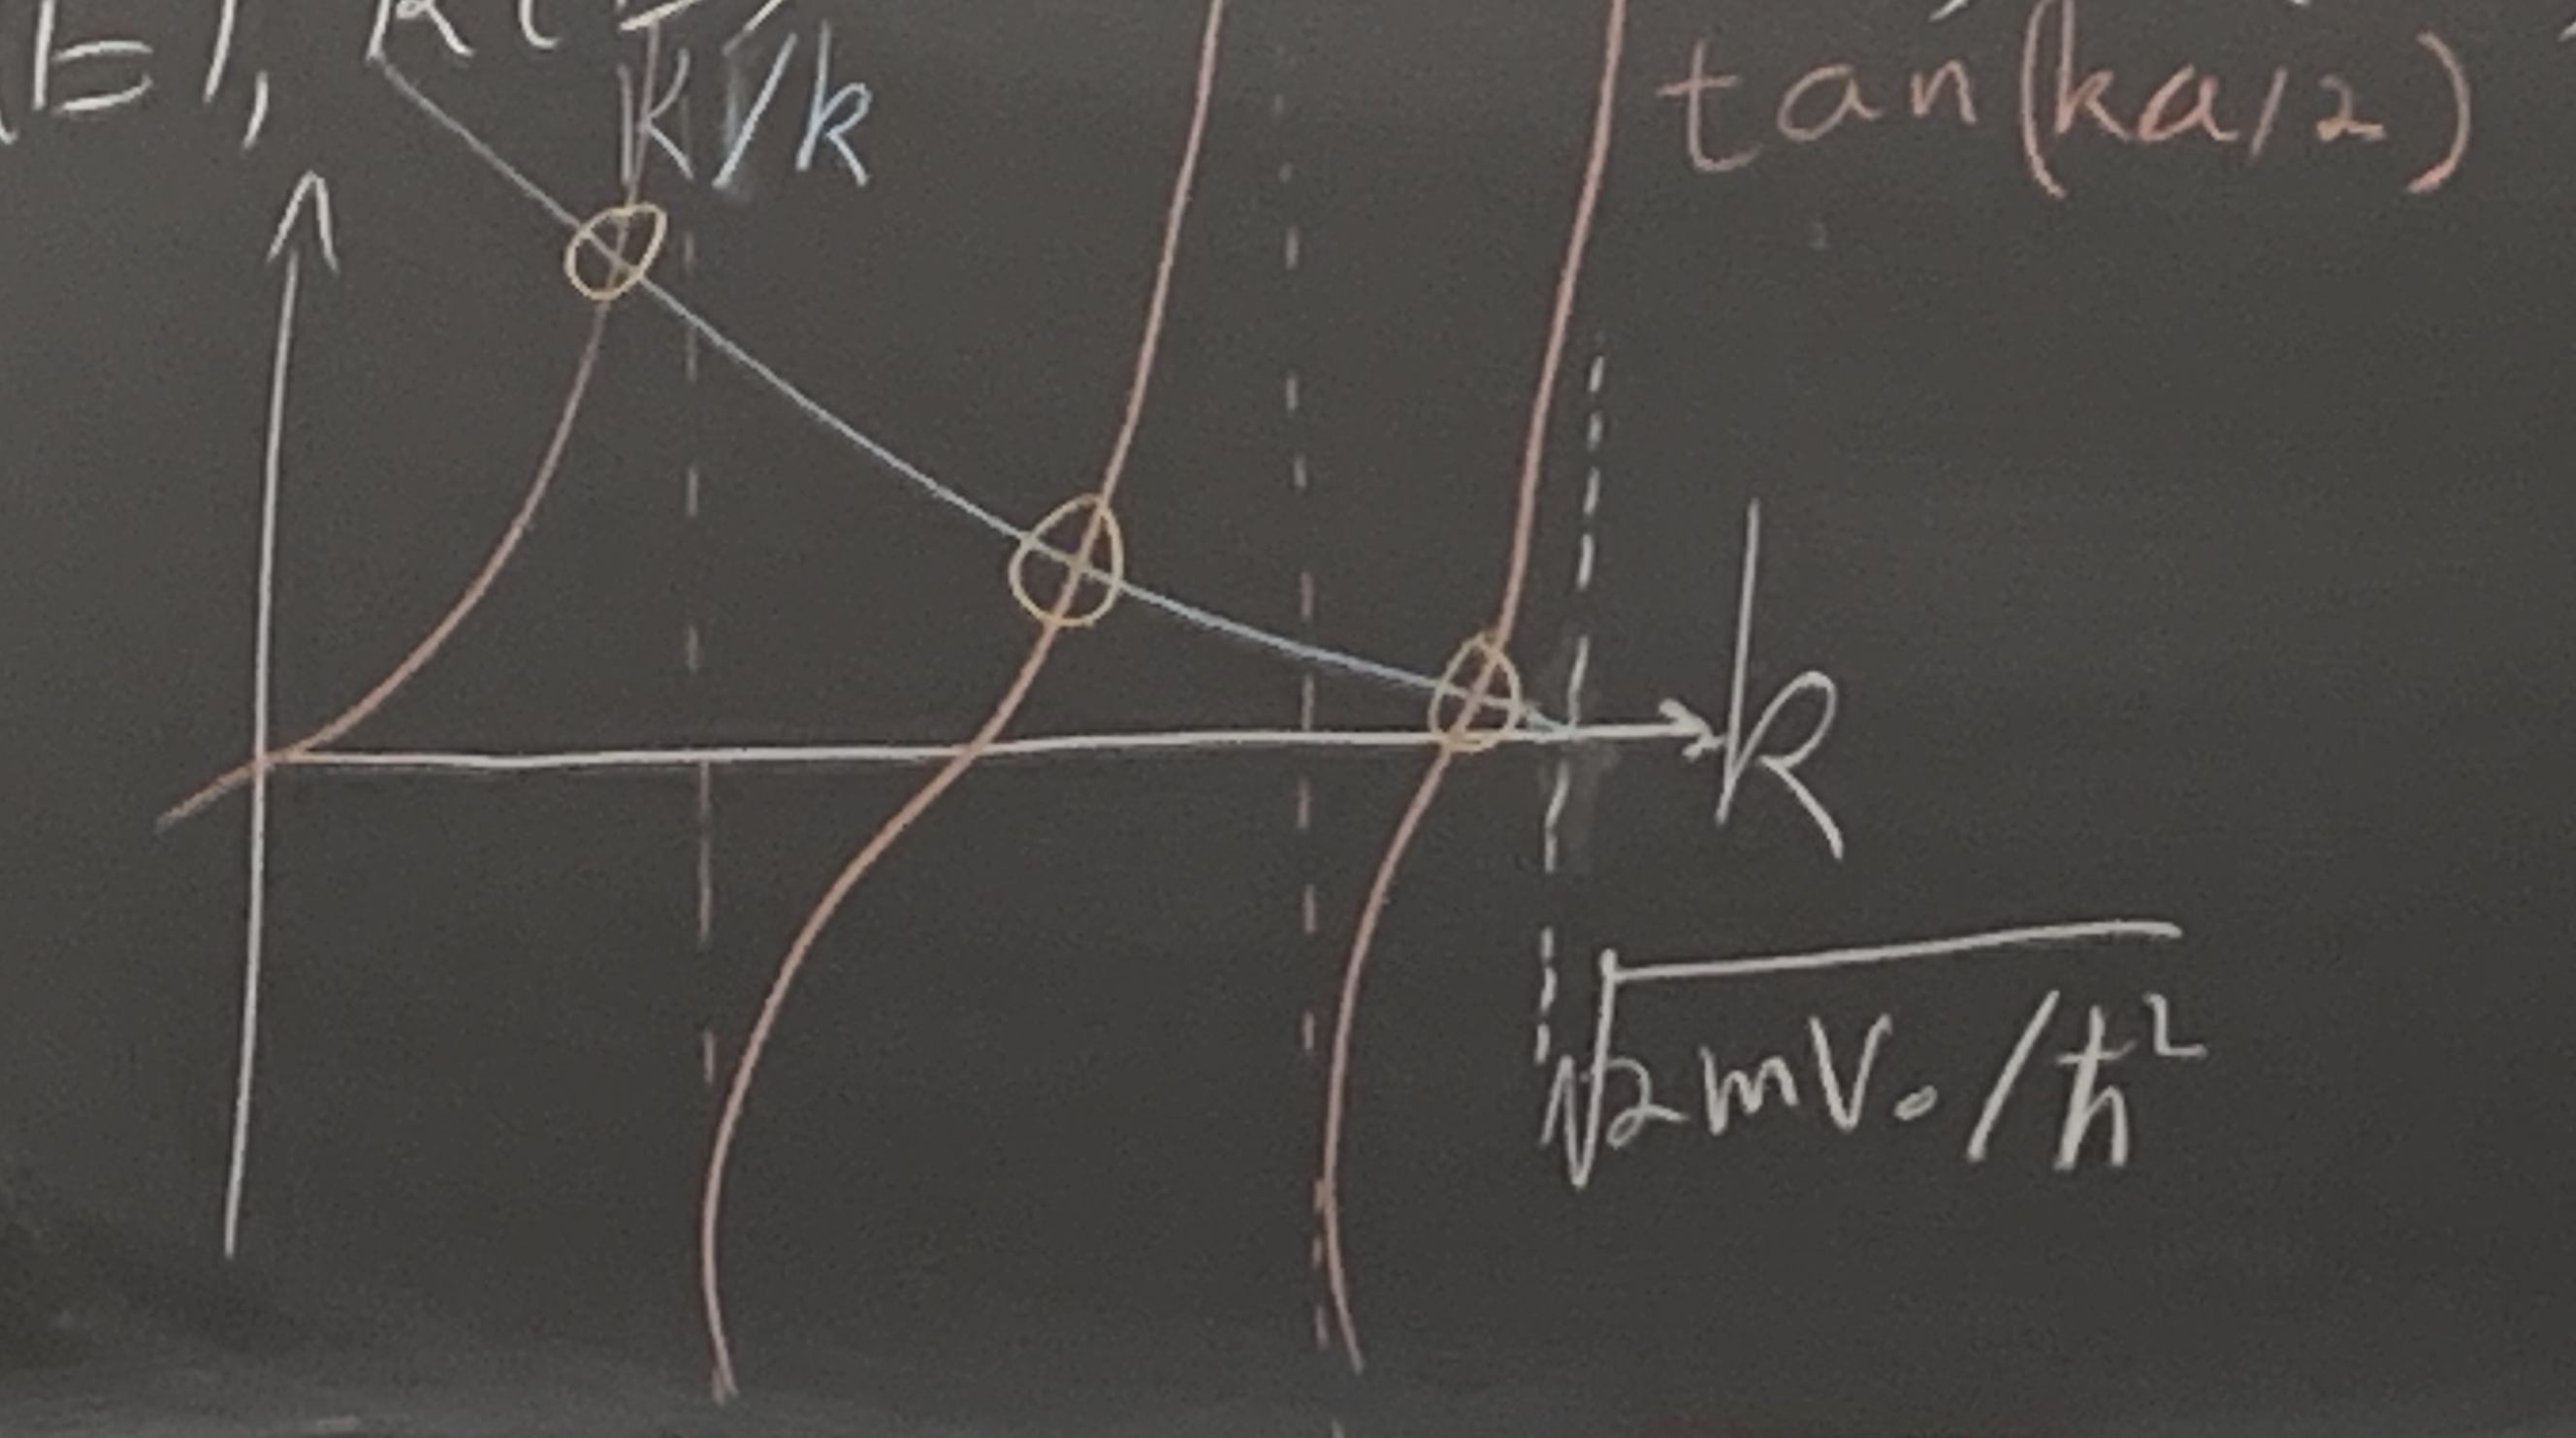
\includegraphics[width=0.5\columnwidth]{figures/lec_28_kappa_vs_k.jpg}
    \caption{$ \tan(ka/2) $ and $ \kappa / k $ plotted as functions of $ k $}
    \label{fig:k_kappa_relation}
\end{figure}

Notice an upper bound on $ k $, implying that these are bound states with energy less than $ V_0 $.

As $ V_0 \to \infty $, $ k \to \infty $ and $ \tan(k a/2) \to \infty $ since $ \cos(k a/2) \to 0 $. Now the upper bound on $ k $ vanishes, so there will be an infinite number of solutions,
\begin{equation}
    k_n = \frac{(2n+1) \pi}{a} \implies E_n = \frac{\hbar^2}{2m} k_n^2
\end{equation}

If we look at the boundary condition on $ \varphi_- $, we get a cotangent function, which gives the form $ k_n = \frac{2 n\pi}{a} $. If we look at both even and odd solutions, we get that $ k_m = \frac{m \pi}{a} $.

Let's now look in the limit where $ E \to 0 $, $ k \to 0 $ and $ \kappa \to 0 $ accordingly.
\begin{equation}
    \tan(k a/2) \approx k a/2 = \kappa / k
\end{equation}
so (if we let $ a/2 = 1 $ and $ \hbar^2 / 2m = 1 $)
\begin{equation}
    E = \sqrt{V_0 - E}
\end{equation}
which comes from $ k^2 = \kappa $.
\begin{equation}
    E = V_0 - E^2 < V_0
\end{equation}
so at least one solution always exists no matter how small $ V_0 $ is. Graphically, the leftmost solution will slide down the tangent curve toward $ 0 $. For example, if we have a one-dimensional wire, if there is a defect, no matter how small, we will have a state trapped at the defect. This tells us that there is no true electrical conductivity in one dimension.



\end{document}
